%%%%%%%%%%%%%%%%%%%%%%%%%%%%%%%%%%%%%%%%%%%%%%%%%%%%%%%%%%%%%%
%                     Gerardo Mazzei                         %
%  based on Luke Van Hulle's and Christian Schaefer's thesis %
%%%%%%%%%%%%%%%%%%%%%%%%%%%%%%%%%%%%%%%%%%%%%%%%%%%%%%%%%%%%%%

% The main thesis document

%% These arara commands are placed here to show the order of operations required to compile this document. If you want to use arara with the subfiles package then these commands will also need to go in every included file. Arara is convenient for multiple workstation compilation and when you need other people to be able to build your document but so far I am not very satisfied with the error reports it generates. Hopefully version 4.0 has a little more documentation and fixes these problems.

% arara: pdflatex
% arara: nomencl
% arara: bibtex
% arara: pdflatex

\documentclass[ 12pt, letterpaper, twoside, openany]{book}

%These files define a lot of the formatting and commands used throughout the document
% 02_Inputs.tex
% the packages are put in a seperate file to help keep the main.tex file clean

% To use the fontec package properly make sure the cm-super
% package is installed for MikTex.
% https://docs.miktex.org/2.9/manual/pkgmgt.html
\usepackage[T1]{fontenc}
\usepackage{fancyhdr}

\usepackage[textwidth=65pt]{todonotes}
\usepackage{siunitx} % provides formating for numbers with SI units

\usepackage{subfiles} % For being able to compile the subfiles on their own

%For math related stuff
\usepackage{amsmath}
\usepackage{systeme}

\usepackage{lipsum} % Used for making dummy text

\usepackage{booktabs} % Makes tables better
\usepackage{tablefootnote} % for making footnotes in tables

% used for loading graphics
\usepackage{graphicx}
\graphicspath{{Figures/}}
% used for making sub-figures
\usepackage{subfig}
%used for placing text over images
\usepackage[percent]{overpic}

% Helps with making arrow with overpic
\usepackage{pict2e}

% use the \layout command and compile to show margins
\usepackage{layout}

% For figures with text wrapped around them
\usepackage{wrapfig}
% For tables with longer text, where manipulating space may be a pain
\usepackage{tabu}
% For special formating of lists
\usepackage{enumitem}

\usepackage{nomencl}
\makenomenclature
\renewcommand{\nomname}{Symbols and Acronyms}

% From https://www.sharelatex.com/learn/Nomenclatures
\usepackage{etoolbox}
\renewcommand\nomgroup[1]{%
  \item[\bfseries
  \ifstrequal{#1}{S}{Symbols}{%
  \ifstrequal{#1}{A}{Acronyms}}%
]}
 
% This will add the units to nomenclature
%----------------------------------------------
\newcommand{\nomunit}[1]{%
\renewcommand{\nomentryend}{\hspace*{\fill}#1}}
%----------------------------------------------

\usepackage{titlesec}

\titleformat{\chapter}
  {\huge\bfseries} % format
  {\thechapter \enspace}   % label
  {0pt}             % sep
  {\huge}           % before-code

% Change the plain style used by chapters as shown on page 7 of
% the fancyhdr manual: http://texdoc.net/texmf-dist/doc/latex/fancyhdr/fancyhdr.pdf
\fancypagestyle{plain}{%
\fancyhf{} % clear all header and footer fields
\fancyhead[LE, RO]{\thepage} %RO=right odd, RE=right even
\renewcommand{\headrulewidth}{0pt}
\renewcommand{\footrulewidth}{0pt}}

\setlength{\headheight}{14.5pt} % to prevent the \headheight warning
\fancyhf{}

%%% Use these four to make it look like a nice book
\fancyhead[LE, RO]{\thepage} % Page number
\fancyhead[LO, RE]{\slshape \leftmark} % Chapter number and name
\renewcommand{\chaptermark}[1]{\markboth{\thechapter.\ #1}{}}
\renewcommand{\headrulewidth}{1pt}

%%% Use these two make it fit the University Guidelines
%\fancyhead[RE, RO]{\thepage}
%\renewcommand{\headrulewidth}{0pt}


% set the margins to the UW-Madison's standard
\usepackage[left=1.3in,
                        top=1.3in,
                        right=1.1in,
                        bottom=1.1in,
                        marginparwidth=65pt]
                        {geometry}

\usepackage[backend=bibtex, sorting=none,maxbibnames=99]{biblatex} %References are numbered per order of use in the text as opposed to alphabetically (default)
\addbibresource{BibTex/prelim.bib}

\usepackage[numbered]{matlab-prettifier} % Used to import MATLAB code 
\usepackage{epigraph} % Only used in the SciSlice chapter
%\usepackage{pdfpages} % Used to import pdfs onto the document

%------------------------------------------------------------------------------------		
%Hyperlinks and PDF Settings
\usepackage[
	bookmarksopen =false, 				% Display bookmarks when the document is opened
	pdftoolbar =true, 					% Display Acrobat reader toolbar
	bookmarksnumbered =true,			% Display section numbers
	pdfpagelabels = false, 				% Display original page numbers
	%plainpages = false, 				% Blank pages
	hyperfootnotes=true,
	pdfpagelayout = TwoPageRight, 		% Open PDF as 2 sided when opened	
]{hyperref}

%Hyperref format
\hypersetup{
	colorlinks=true,	% Hyperlinks are colored
	linkcolor=blue,		% Color of internal links (within document)
	citecolor=blue,	    % Color of internal links to the Reference page (within document)
	urlcolor=blue,		% Color of URLs (external) - default is magenta.
	pdftitle = {Predicting mechanical properties of FFF parts through Machine Learning},
	pdfsubject = {Prelim 2020},
	pdfauthor = {Gerardo A. Mazzei Capote},
	pdfkeywords = { },	
}
\usepackage{url}
%%%%%%%%%%%%%%%%%%%%%%%%%%%%%%%%%%%%%%%%%%%%%%%%%%%%%%%%%%%%%%%%%%%%%%%%%%%%%%%%%%%%%%%%%%%%%%%%%%%%%%%%%%%%%%%%%%%%%%%%%%%%%%%%%%%%%%%%%%%%%%%%

% Präamble: Ploteinstellungen

%%%%%%%%%%%%%%%%%%%%%%%%%%%%%%%%%%%%%%%%%%%%%%%%%%%%%%%%%%%%%%%%%%%%%%%%%%%%%%%%%%%%%%%%%%%%%%%%%%%%%%%%%%%%%%%%%%%%%%%%%%%%%%%%%%%%%%%%%%%%%%%%

% Für Plots
\usepackage{pgfplots}
\usepackage{pgf}
\usepackage{chemfig}
% Version
\pgfplotsset{compat=1.9}
\usepgfplotslibrary{patchplots}

% Hauptgitter
\pgfplotsset{major grid style={gray}}

% Nebengitter
%\pgfplotsset{minor grid style={dashed,red}}

% Alles inerhalb von Tikz-Umgebung in SF
\tikzset{ every picture/.style = {font=\rmfamily} }

% Groupplots erlauben
\usepgfplotslibrary{groupplots}

\usetikzlibrary{patterns,chains}

%Für Bilder
\usepackage{tikz}
  
\usetikzlibrary{shapes.geometric}% für Ellipse
%\tikzset{
%  pfeil/.style={stealth-},
%  beschr/.style={remember picture,overlay,font=\small}}
%\newcommand\mrahmen[3][]{%
%  \tikz[baseline,remember picture]
%    \node[anchor=base,inner sep=2pt,draw=#2,#1]{$\displaystyle#3$};}
%\colorlet{mfarbe}{red}
%\newcommand\sbinom[2]{\genfrac{}{}{0pt}{}{#1}{#2}}

\usetikzlibrary{calc,positioning,arrows}
\usetikzlibrary{fit}

%Für Plots
\usepackage{tikzscale}
\usepackage{filecontents}

%Wegen Overwriting
\usepackage{silence} 
\WarningFilter{latex}{Overwriting file}

\tikzset{ every pin/.style={rectangle,rounded corners=3pt,font=\small}, small dot/.style={fill=black,circle,scale=0.3}}

% \pgfplotsset{
  % tick label style = {font=\sansmath\sffamily},
  % every axis label = {font=\sansmath\sffamily},
  % legend style = {font=\sansmath\sffamily},
  % label style = {font=\sansmath\sffamily}
% }

% PEC Style Graph
%%%%%%%%%%%%%%%%%%%%%%%%%%%%%%%%%%%%%
%Globale Definition der Einträge!
\pgfplotsset{
    cycle list={PEC_red,mark=triangle,line width = 1pt,smooth\\
                black,mark=square,line width = 1pt,smooth\\
                gray,mark=triangle,line width = 1pt,smooth\\
                PEC_red2,mark=square,line width = 1pt,smooth\\
                },
}
%%%%%%%%%%%%%%%%%%%%%%%%%%%%%%%%%%%%%%%%%%%%%%%%%%%%%%%%%%%%%%%%%%%%%%%%%%%%%%%%%%%%%%%%%%%%%%%%%%%%%%%%%%%%%%%%%%%%%%%%%%%%%%%%%%%%%%%%%%%%%%%%

% Präamble: Farben und Einstellungen der Farben

%%%%%%%%%%%%%%%%%%%%%%%%%%%%%%%%%%%%%%%%%%%%%%%%%%%%%%%%%%%%%%%%%%%%%%%%%%%%%%%%%%%%%%%%%%%%%%%%%%%%%%%%%%%%%%%%%%%%%%%%%%%%%%%%%%%%%%%%%%%%%%%%

% Farben laden
\usepackage{xcolor}
\usepackage{colortbl}

% Farben selbst definierten
\definecolor{grau}{rgb}{0.9,0.9,0.9}
\definecolor{dunkelgrau}{rgb}{0.8,0.8,0.8}

\definecolor{gelb}{rgb}{1,1,0}

\definecolor{rot}{rgb}{1,0,0}

\definecolor{blau}{rgb}{0.2,0.2,1}

\definecolor{FAU_blau}{RGB}{0,60,100}
\definecolor{FAU_grau}{RGB}{140,140,140}

\definecolor{mygreen}{RGB}{28,172,0} % color values Red, Green, Blue
\definecolor{mylilas}{RGB}{170,55,241}
\definecolor{myturkis}{RGB}{0,191,255}

\definecolor{PEC_red}{RGB}{153,0,0}
\definecolor{PEC_red2}{RGB}{172,8,9}
%\definecolor{hellgrau}{rgb}{0.95,0.95,0.95}
%\definecolor{dunkelrot}{rgb}{0.95,0.0,0.4}

\usepackage{footnote}
\renewcommand*{\thefootnote}{\alph{footnote}}


% To make the Structure section work in TexMaker it needs to see
% the \include command, but the subfiles package needs \subfile
% so I changed \include to just call \subfile.
\renewcommand{\include}[1]{
        \subfile{#1}}

\begin{document}
        \frontmatter
        		\pagenumbering{gobble} %No page number in front matter
                % cover.tex
% Cover Pages

\documentclass[main.tex]{subfiles}
\begin{document}

\begin{titlepage}
	\begin{center}
		\vspace{1cm}
		{\scshape\Huge\textbf{Predicting mechanical properties of FFF parts through Machine Learning} \par}
		\vspace{1cm}
		{\LARGE\textbf{Gerardo A. Mazzei Capote} \par}
		\vspace{1cm}
		{\Large A preliminary report submitted in partial fulfillment of \par 
				the requirements for the degree of \par}
		\vspace{1cm}
		{\LARGE\textbf{Doctor of Philosophy} \par}
		{\LARGE\textbf{(Mechanical Engineering)} \par}
		\vspace{1cm}
		{\Large at the \par}
		\vspace{0.5cm}
		{\scshape\LARGE\textbf{ University of Wisconsin-Madison} \par}
		\vspace{0.5cm}
		{\Large 2020 \par}
		\vfill
		{\large May 2020}		%MODIFY DATE
	\end{center}
\end{titlepage}

\pagestyle{empty}
\cleardoublepage
\setcounter{page}{1}

\chapter*{Approval}
%\thispagestyle{fancy}
The following preliminary report, \textbf{Predicting mechanical properties of FFF parts through Machine Learning}, developed at the \textbf{University of Wisconsin-Madison}
has been approved by:
\vspace{2cm}

\noindent
\makebox[7cm]{\hrulefill} \hfill\makebox[4cm]{\hrulefill}
\par\noindent
\textit{Signature} \hfill\textit{Date}\hspace{3cm}
\vspace{5 mm}
\par\noindent
\textbf{Professor Tim A. Osswald}
\par\noindent Department of Mechanical Engineering
\par\noindent College of Engineering
\par\noindent University of Wisconsin-Madison

\cleardoublepage

\end{document}



                \addcontentsline{toc}{chapter}{Front Matter}
                \pagenumbering{roman}
                % abstract

\documentclass[main.tex]{subfiles}
\begin{document}
\setcounter{page}{1}
\chapter*{Abstract}
Fused Filament Fabrication (FFF) is arguably the most widely available Additive Manufacturing technology at the moment. Offering the possibility of producing complex geometries in a compressed product development cycle and in a plethora of materials, it comes as no surprise that FFF is attractive to multiple industries, including the automotive and aerospace segments. However, the high anisotropy of parts developed through this technique implies that part failure prediction is extremely difficult \textemdash a requirement that must be satisfied to guarantee the safety of the final user. Application of a Failure Criterion to predict part failure can solve this issue. However, a large number of mechanical tests performed under a variety of loading conditions are required to populate the parameters of the function that describes the failure envelope - a process that is extremely time consuming. This research proposal describes a method by which the development of the failure surface can be streamlined, and the number of mechanical tests can be significantly reduced. 
 
\vspace{10mm} %10mm vertical space
\textbf{Keywords:} FFF, FDM, Failure Criteria, Mechanical Testing, Machine Learning.

\vfill %Send copyright notice to bottom of the page
\begin{center}
Copyright~\textcopyright: Gerardo A. Mazzei Capote (2020)

\emph{All rights reserved}	
\end{center}
\end{document}                
                \addcontentsline{toc}{section}{Abstract}
                %\include{acknowledgments}
               % \addcontentsline{toc}{section}{Acknowledgments}
                \renewcommand{\contentsname}{Table of Contents}
                \tableofcontents
                
                \printnomenclature
                \addcontentsline{toc}{section}{Nomenclature}
                \listoffigures
                \addcontentsline{toc}{section}{\listfigurename}
               \listoftables
               \addcontentsline{toc}{section}{\listtablename}
               \cleardoublepage
                               
        \mainmatter
                \pagestyle{fancy} % Needed again because it is turned off in some
                                                  % previous sections.                
                % introduction.tex

\documentclass[main.tex]{subfiles}
\begin{document}
	%The next two lines ensure that the Introduction is a unnumbered chapter that shows up in the index
\chapter*{Introduction}\label{ch:intr}
\addcontentsline{toc}{chapter}{Introduction} \markboth{Introduction}{}
%Chapter body
\emph{Additive Manufacturing} (AM) is an umbrella term that encompasses all fabrication techniques where the final geometry of the part is obtained through superposition of material in a layer-by-layer basis \cite{Gibson2015}. Developed in the 1980s, this manufacturing technique permits immensely shorter part development cycles, since the transition from a 3D \emph{Computer Aided Design} (CAD) to part fabrication only requires one intermediate step: the use of a slicing engine that converts the geometry of the object into machine instructions \cite{Gibson2015}. For this reason, AM technologies were initially employed exclusively for prototype development and were referred to as \emph{Rapid Prototyping techniques} (RP). However, recent innovations in the field have caused AM to be considered as a legitimate manufacturing technology since it is also capable of reproducing complex geometries unattainable through traditional methods \cite{Gibson2015}.

While offering great advantages over traditional part fabrication methods, AM comes with its own set of limitations and disadvantages: First and foremost, the use of a stratified build approach tends to produce extremely anisotropic parts. Secondly, the geometric accuracy of the object produced is highly dependent of process parameters, particularly, the thickness of the layers. Finally, as of the time of this writing, AM lacks the standardization and scrutiny that are associated to most traditional manufacturing techniques \cite{Gibson2015}.  

\emph{Fused Filament Fabrication} (FFF), also known under the trademark \emph{Fused Deposition Modeling} (FDM\texttrademark), represents perhaps the most prevalent AM technique in the market due to the advent of low-cost, desktop 3D printers in the early 2010s \cite{Capote2017}. Due to the broad availability of machines and relatively low costs of material, there is a surging interest in optimizing FFF to produce small batches of end-user grade parts. Success stories are varied, but examples include vacuum form molds, fixtures, jigs, and tools used to aid assembly lines in the automotive industry \cite{Hartman2014, VanHulle2017,deVries2017}. However, this technology still faces the challenges and limitations that currently affect the field of AM as a whole. Namely, anisotropy introduced through the layer-by-layer build approach makes it difficult to assess the expected mechanical behavior of FFF parts when subjected to important mechanical stresses \cite{Capote2017}. For these reasons, multiple attempts have been made to characterize the anisotropy of FFF manufactured objects, such as the studies performed by Koch \emph{et al.} \cite{Koch2017} and Rankouhi \emph{et al.} \cite{Rankouhi2016}, which show that the ultimate tensile strength of FFF coupons is sensitive to process parameters such as the layer thickness and, in particular, the orientation in which the plastic strands are laid during the build process -henceforth referred to as the bead orientation. Literature related to preventing failure through predictive methods in the design stages is scarce. However, a handful of publications exist where this issue was solved through the application of a failure criterion. The reach of this methodology has been fairly limited, given the difficulty of using commercially available AM machines to produce test coupons with unconventional bead orientations necessary to populate the failure surface, as well as the limitations inherent to development of failure criteria. Examples include the developments of failure envelopes for \emph{Polyamide 12} (PA12) used in \emph{Selective Laser Sintering} (SLS) and Multi-Jet Fusion (MJF) \cite{Obst2018, Osswald2020}, and more importantly for this body of work, a failure surface for \emph{Acrylonitrile Butadiene Styrene} (ABS) used in FFF \cite{MazzeiCapote2019}. For the latter, certain test specimens in unconventional configurations had to be produced using a unique off-axis 3D printer developed in-house. In both cases, the researchers utilized a FC that incorporates stress interactions into the calculations of the failure surface, a feature that more recognized criteria, such as the Tsai-Wu model fail to take into account \cite{Osswald2017a}.

Additional predictive tools have been pushed to the forefront of engineering applications given recent developments in the fields of statistics, data science, artificial intelligence, worldwide connectivity, and computational hardware. These tools allow designing intelligent systems that can, among many things, detect and correct problems during a production run, identify trends, and more importantly for the objective of this work, predict outcomes or perform classification tasks. These tools have been grouped under the \emph{Machine Learning} (ML) moniker, and are currently being exploited by large companies to make sense of large clusters of data. Machine Learning tools thrive in cases where the inputs and outcomes of a particular phenomena or task are known, but connecting the two through an explicit set of rules or relationships can result extremely complex and time consuming \cite{Chollet2018} because, in simple terms, ML models are trained, as opposed to explicitly programmed. Their broad range of applications has caused its use to trickle into other segments of engineering, usually in the form of \emph{Neural Networks} or \emph{Support Vector Machines} performing a variety of regression analysis or classification tasks. The field of AM is no stranger to the ML topic. Interest in the subject has been remarked by several authors \cite{Qi2019, Razvi2019, Meng2020}, and it has even been successfully applied to predict certain properties of AM parts produced under various techniques \cite{Qi2019, Razvi2019, Meng2020, Sood2012}. 

The set of printing conditions that lead to an optimal part in terms of mechanical properties aren't still fully comprehended and result in extremely complex, multi-variable relations. However, an FFF machine with in-line sensors that allowed monitoring a variety of process-variables, as well as data generated from mechanical tests and ancillary experiments would constitute a perfect case for deployment of a Machine Learning system capable of predicting the mechanical properties of the finished part. In this manner, this work proposes to apply ML techniques to the FFF process in order to predict mechanical properties according to in-line measurements. Chapter \ref{ch:bg} will introduce basic concepts used throughout this work; Chapter \ref{ch:oocrit} will provide details pertaining to failure prediction of AM parts through failure criteria, focusing on previous work performed by the author on failure prediction for FFF parts; finally, Chapter \ref{ch:proposal} will supply information pertaining to why and how a ML solution is of interest, as well as displaying preliminary results available at the time of this writ.

%Nomenclature introduced in this chapter:
\nomenclature[A]{AM}{Additive Manufacturing}% 
\nomenclature[A]{RP}{Rapid Prototyping}%
\nomenclature[A]{CAD}{Computer Aided Design}%
\nomenclature[A]{FDM}{Fused Deposition Modeling\texttrademark}
\nomenclature[A]{FFF}{Fused Filament Fabrication}%
\nomenclature[A]{FC}{Failure Criterion}%
\nomenclature[A]{ABS}{Acrylonitrile Butadiene Styrene}%
\nomenclature[A]{PA12}{Polyamide 12}%
\nomenclature[A]{AI}{Artificial Intelligence}%

\end{document}
                % background.tex
\documentclass[main.tex]{subfiles}
\begin{document}
\chapter{Background} \label{ch:bg}
\section{Additive Manufacturing}\label{sec:AM} %Section labeling for cross-referencing
\emph{Additive Manufacturing} (AM) technologies had their beginnings in the decade of the 1980s. During this time, various independently developed patents were filed across the globe, describing a process that would construct an object by selectively adding layers of material -as opposed to removing excess matter or deforming mass to obtain a desired shape. This represents the core definition of AM: any technology where the final geometry of the manufactured object is obtained through controlled addition of material qualifies as an Additive Manufacturing technique \cite{Gibson2015}.

Advancements in the fields of computing, \emph{Computer Aided Design} (CAD), and controllers, among other technological developments, were necessary to translate the patents into working prototypes, with some eventually becoming the foundations of commercially successful companies -such as 3D Systems in 1986 and Stratasys in 1989 \cite{Gibson2015,3DSystems,Stratasys2017}. The basic process of AM has remained largely unchanged from its first iteration in the late 80s: First, a computer model of the object is made using CAD software and exported under the .\emph{stl} file format. Afterwards, the part geometry is stratified, or \textquotedblleft sliced\textquotedblright, and translated into machine instructions using a specialized software called \emph{slicing engine}. An AM machine then follows said instructions, commonly referred to as the \emph{toolpath}, to build the object in layers. Finally, the part is available to the user. Depending on either the requirements of the part, or the specifics of the AM technique used, some post-processing may be required \cite{Gibson2015}. A visual representation of the process is shown in Figure~\ref{fig:AM_flow}.

\begin{figure}[h]
	\center
	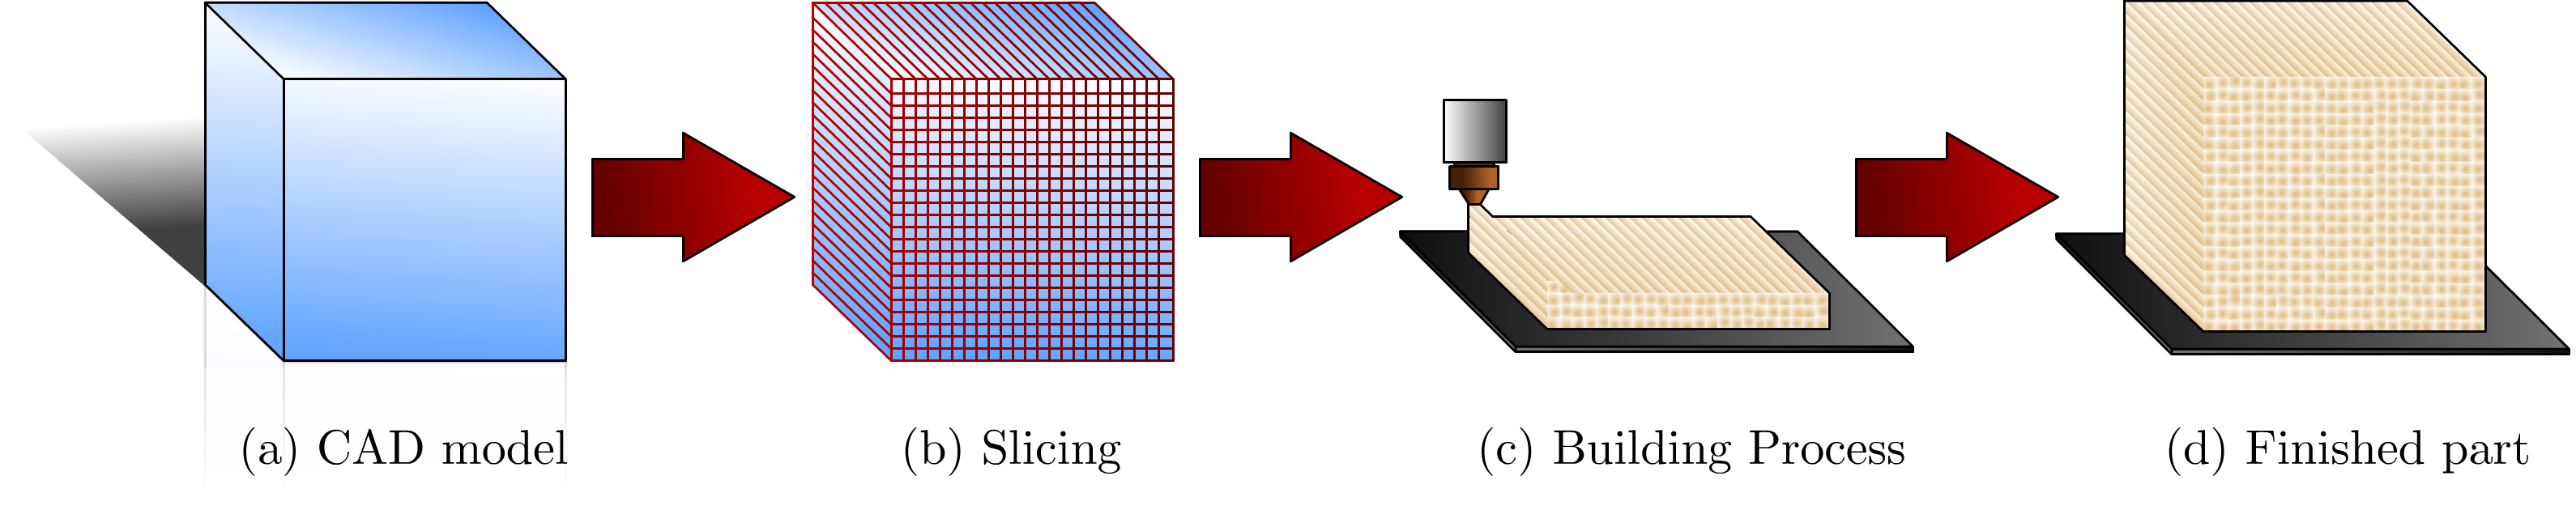
\includegraphics[width=\linewidth]{AM_flowchart_1}
	\caption{Process flow of AM} \label{fig:AM_flow}
\end{figure}
\pagebreak %Used to move the entire paragraph to a new page.
 
While all AM technologies operate on the same basic process flow described above, the specifics of each AM technique vary substantially, ranging from processes that use paper and binder, all the way through metal-based, laser tracing technologies. Since this is a rapidly evolving field, no general consensus exists for classifying the multiple AM processes available as of the time of this writing. However, the classification system proposed under the ASTM/ISO 52900 standard \cite{ASTM52900}, has been somewhat accepted by the field and divides AM technologies as follows:
\begin{enumerate}
	\item \textbf{Binder Jetting}: AM techniques where a binding agent is used to selectively promote cohesion in powder materials -generally gypsum, sand or metallic powders~\cite{ASTM52900,3DHubs2018}.
	\item \textbf{Directed Energy Deposition}: AM processes where a focused thermal energy source (i.e. laser, electron beam, plasma arc) is used to fuse materials as they are being deposited in the build volume. Materials are almost exclusively metals~\cite{ASTM52900,3DHubs2018}.
	\item \textbf{Material Extrusion}: In this type of AM technology, material is dispensed through a nozzle or orifice. Fused Filament Fabrication belongs to this classification. Materials are almost exclusively thermoplastics \cite{ASTM52900,3DHubs2018}.
	\item \textbf{Material Jetting}: AM techniques where build material is deposited selectively in droplets. Materials are usually wax or thermoplastics, but there are examples of metal-based, material jetting techniques \cite{ASTM52900,3DHubs2018}.
	\item \textbf{Powder Bed Fusion}: AM processes where portions of a powder bed are selectively fused through application of thermal energy. \emph{Selective Laser Sintering} (SLS) belongs to this category. Materials are usually thermoplastic polymers or metals \cite{ASTM52900,3DHubs2018}. 
	\item \textbf{Sheet Lamination}: In this type of AM technology, the final part is formed by bonding sheets of material -usually paper or composites \cite{ASTM52900,3DHubs2018}. 
	\item \textbf{Vat Photopolymerization}: In this AM process, a liquid photopolymer is selectively cured by a light source. \emph{Stereolithography} (SLA), arguably the first AM technology, belongs to this category. Due to the nature of this technique, the only materials used are photopolymers \cite{ASTM52900,3DHubs2018}.
\end{enumerate} 

\subsection{Advantages and Disadvantages of AM}\label{subsec:AMAdDis} 
Since AM processes allow a relatively direct conversion of a CAD model into a constructed object, they were originally exclusively used for prototype development. For this reason, they were initially classified as \textquotedblleft \emph{Rapid Prototyping}\textquotedblright~(RP) technologies. This terminology is still used today, however, it is being superseded by \emph{Additive Manufacturing} since its potential to become a proper fabrication technique exists \cite{Gibson2015}. While being capable of quickly jumping from part design to manufacturing is a great advantage, AM has its own set of drawbacks. Table \ref{tab:AM_AdDis} summarizes the most noteworthy set of advantages and disadvantages typical of most AM technologies.

\begin{table}[h]
	\centering
	\caption{Advantages and Disadvantages of Additive Manufacturing}
	\label{tab:AM_AdDis}
	\begin{tabu} to 0.95\textwidth {  X[c]  X[c] }
		\hline
		\textbf{Advantages} & \textbf{Disadvantages} \\ 
		\hline
		Faster product development cycles \cite{Gibson2015} & Part quality highly dependent on process parameters \cite{Gibson2015}\\
		%---------
		No additional tools needed for part fabrication\cite{Gibson2015}&  Stratified build generally results in anisotropic parts \cite{Gibson2015, Capote2017}\\
		%---------
		Cost effective for small batches of parts \cite{Baumers2016,Conner2014,Berman2012}&  Costly for production of more than hundreds of parts \cite{Baumers2016,Conner2014,Berman2012}\\
		\hline
	\end{tabu}
\end{table}   

Out of all the described advantages and disadvantages, the high anisotropy of AM parts is responsible for the slow embrace of AM in highly demanding engineering fields -such as the aerospace and automotive industries. The highly anisotropic mechanical behavior makes it extremely difficult to predict part failure, therefore, it cannot be implemented in engineering applications where catastrophic failure is to be avoided at all costs. Even so, success stories of implementation of AM in industrial environments are abundant. Relatively recent examples include the use of FFF machines to manufacture tools, jigs, and fixtures in a Volkswagen assembly plant in Europe \cite{deVries2017}; production of a complex fuel nozzle injector for the LEAP jet engine, using powder based, metal AM by GE \cite{GEAdditive2016}; and development and production of highly optimized, 3D printed midsoles for high performance running sneakers by companies as large as New Balance and Adidas \cite{NewBalance2016,Matisons2015,Saunders2018}. Note that in the cases presented, the main reason behind the usage of AM was either reduction of expenses associated with producing small batches of parts, or the capability of reproducing a unique and complex geometry. This is a trend that is observed in most of the literature describing implementation of AM into industrial scenarios.

While the advantages and disadvantages described here cover the field of AM as a whole, each technique comes with its own set of pros and cons that may make it the preferred method to reproduce a particular product or geometry. This work, however, focuses solely on FFF. The specifics of this process are described in detail in Section~\ref{sec:FFF}.

\section{Fused Filament Fabrication}\label{sec:FFF} 
\emph{Fused Filament Fabrication}~(FFF) is an AM technology where the final geometry of the part is obtained through controlled extrusion of a liquid, self-hardening material -usually a thermoplastic polymer in molten state \cite{Gibson2015}. Originally developed by Stratasys in the 1980s under the still trademarked ~\emph{Fused Deposition Modeling}~(FDM\texttrademark) moniker, it has recently become one of the most widely used AM techniques due to the advent of low-cost, desktop FFF machines in the early 2010s caused by the expiration of key patents from Stratasys \cite{Gibson2015,Capote2017}. 

\subsection{The FFF process}\label{ssec:FFFmach}
At its core, the typical FFF machine consists of a heated build surface commonly referred to as a \emph{build plate}, a specialized tool known as a \emph{printhead}, and the fabrication material -supplied in the form of spools of thermoplastic polymer filament. The printhead is itself composed of a heating element, a nozzle, and some form of driving mechanism that pushes the filament downward. As the thermoplastic material is moved through the heated chamber, polymer melt is formed and extruded through the opening at the tip of the nozzle, producing a \emph{bead}. The molten polymer can then be deposited upon the build plate, where controlled movements of the printhead and the fabrication surface gradually construct the final geometry of the part in a layer-by-layer build approach~\cite{Gibson2015}. The typical setup of an FFF machine can be seen in Figure \ref{fig:machconfig}. In this example, the printhead moves in the \emph{x-y} plane, while the build plate moves in the \emph{z} direction. 
 
\begin{figure}[h]
	\center
	\subfloat[FFF printhead cross section\label{fig:FFFnoz}]{%
		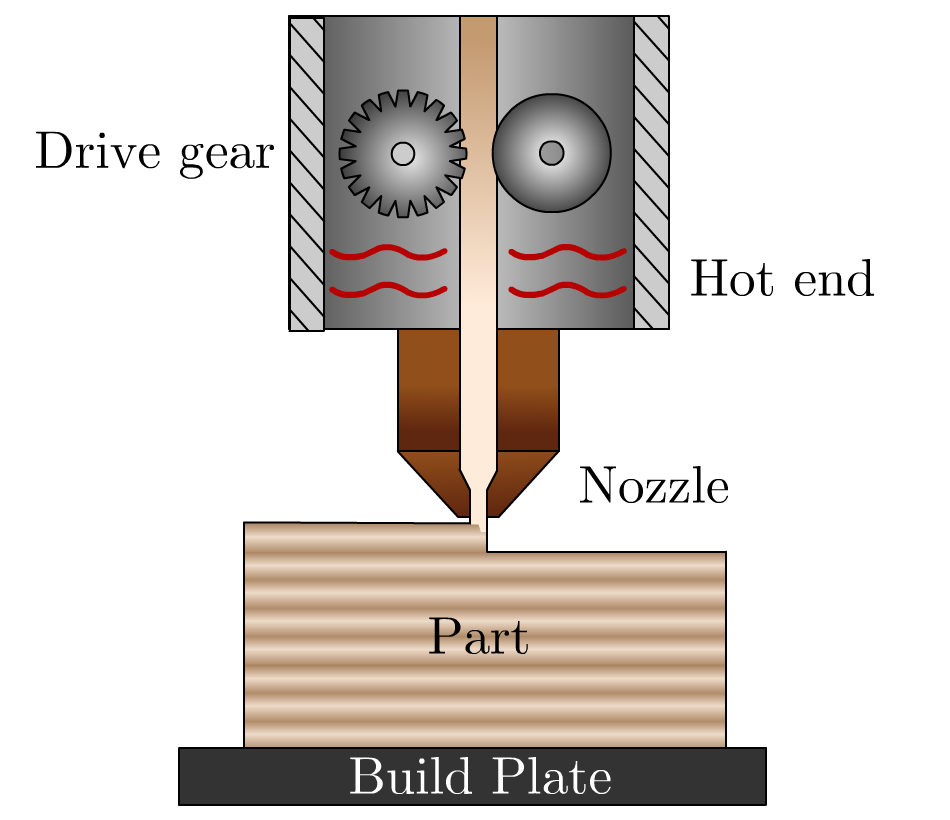
\includegraphics[height=6cm, keepaspectratio]{nozzle}
		}
	\hfill
	\subfloat[Typical FFF machine\label{fig:FFFmach}]{%
		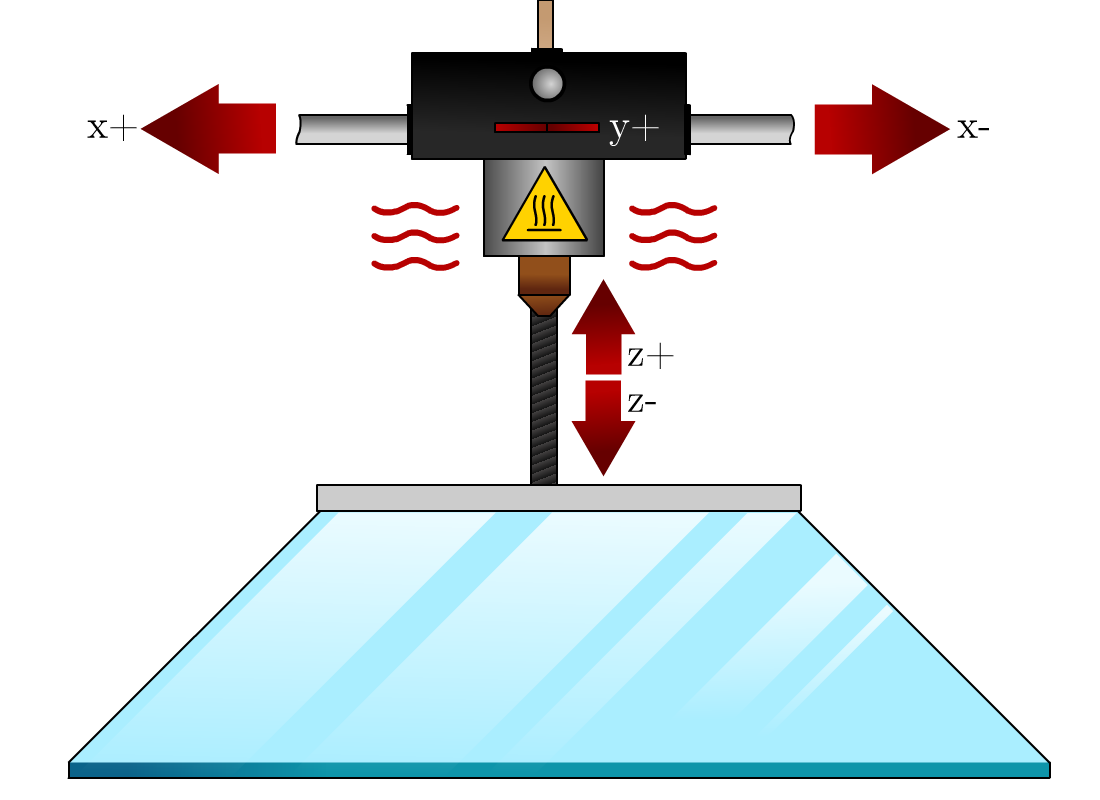
\includegraphics[height=6cm, keepaspectratio]{printer_layout}
		}
	\caption{The basic FFF machine configuration} \label{fig:machconfig}
\end{figure}
Like all AM technologies, the FFF process starts in a computer with a CAD model converted to the \emph{.stl} file format. The geometry is then translated to machine instructions through a \emph{slicing engine}, where the user inputs a plethora of process parameters that include nozzle and build plate temperatures, print speed, layer thickness, and build orientation. Finally the \emph{toolpath} is executed by the FFF printer, building the object in a layer-by-layer basis \textendash~sometimes referred to as \emph{2.5D} printing~\cite{Gibson2015, VanHulle2017}. Figure \ref{fig:FFFflow} shows an abridged version of the process. The \emph{z} axis indicates the intended build direction. Note how some of the finer details in the original CAD file are lost in the printed part \textendash~due in part to the layer height and build orientation selected.

\pagebreak
\begin{figure}[h]
	\center
	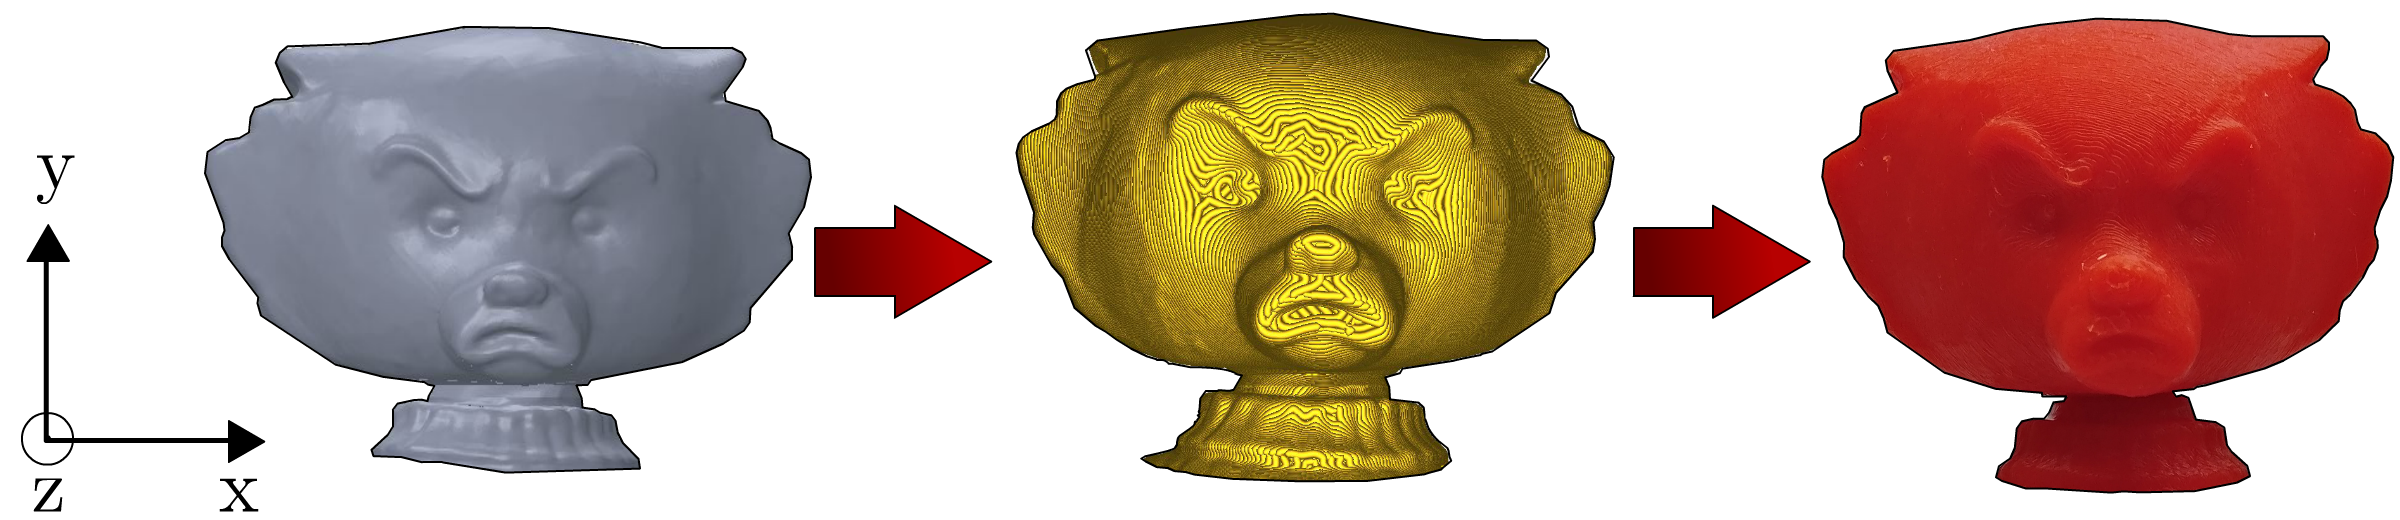
\includegraphics[width=0.95\textwidth]{FFFflow}
	\caption{Model, toolpath and final part in the FFF process} \label{fig:FFFflow}
\end{figure}

The process is capable of producing complex geometries that would be otherwise hard to reproduce through other polymer processing techniques, such as injection molding. However, it is bound by the disadvantages described in Section \ref{subsec:AMAdDis}, as well its own unique set of drawbacks. Namely:

\begin{itemize}
	\item The circular orifice in the nozzle makes FFF incapable of reproducing sharp corners, limits the size of the smallest reproducible feature, and causes the final part to be filled with voids \textendash originating in the junction of round beads. These problems can be seen in Figure \ref{fig:FFFpartprob}: On the left, a comparison of a 90$^\circ$ corner planned in the toolpath and the final geometry of the printed bead is shown. Note the rounded nature of the turn. On the right, a cross section of an FFF part obtained through \emph{Micro Computer Tomography} ($\mu$CT) shows the voids that form during the printing process.
	\begin{figure}[h]
		\center
		\subfloat[FFF toolpath vs. printed bead\label{fig:FFFbead}]{%
			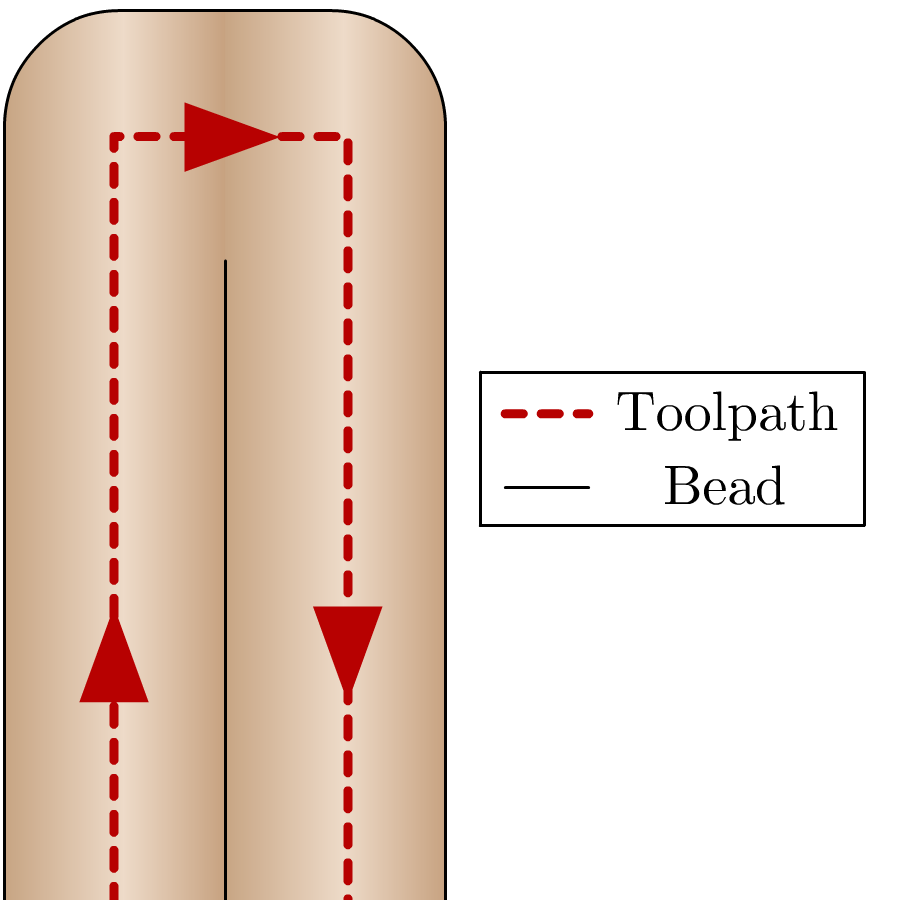
\includegraphics[height=6cm, keepaspectratio]{Toolpath}
		}
		\hfill
		\subfloat[Cross section of an FFF part\label{fig:FFFuCT}]{%
			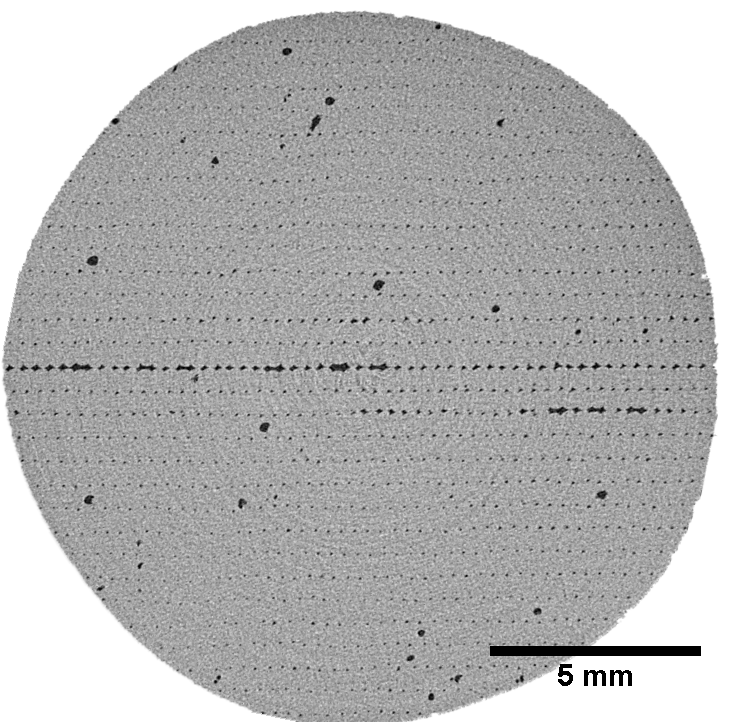
\includegraphics[height=6cm, keepaspectratio]{uCT_FFF}
		}
		\caption{Typical FFF part mesostructure and its origin} \label{fig:FFFpartprob}
	\end{figure}
	\item The junction of adjacent beads behaves akin to a polymeric weld, and has inferior mechanical properties than the bulk material \cite{Capote2017}. This, coupled with the aforementioned voids which can act as stress concentrators, causes FFF parts to behave in extremely anisotropic manner with diminished mechanical performance when compared to analogous parts obtained through traditional polymer processing technologies \textendash~such as injection molding \cite{Capote2017}.
\end{itemize}

This last disadvantage is responsible for the slow embrace of FFF as a proper manufacturing technique: the high anisotropy of FFF parts imply that predicting part failure becomes extremely difficult and thus, proper part design that guarantees safe operation of the object under important loads is hard to achieve.  For this reason, efforts to characterize the mechanical behavior of FFF parts have existed since as early as the 1990s. Recent examples are presented in Section \ref{ssec:mechPropFFF}.

\subsection{Mechanical Properties of FFF parts}\label{ssec:mechPropFFF}

Efforts have been made to characterize the mechanical anisotropy of FFF parts. However, due to the lack of testing standards and problems during toolpath planning, most studies focus solely in the tensile mechanical performance of FFF coupons.

Studies performed by Koch \emph{et al.} \cite{Koch2017} and Rankouhi \emph{et al.} \cite{Rankouhi2016} indicate that the final tensile properties of FFF coupons are particularly sensitive to bead orientation and proper mass output through the nozzle. Other process parameters, such as the layer thickness, have varying degrees of impact upon the final tensile strength of the part. In both studies, tensile coupons were printed with bead orientations of 0$^\circ$, 45$^\circ$ and 90$^\circ$ in the \emph{x-y} plane. Results showed that in all the experimental conditions selected, a 0$^\circ$ orientation always behaved closer to the bulk material, whereas a 90$^\circ$ sample always had significantly lower tensile strengths. The 45$^\circ$ samples sat between both extremes. It is important to note that in both studies, toolpath manipulation was necessary to avoid premature failure of the coupons due to stress concentrators originating in void formation due to the elliptical nature of the beads. Figure \ref{fig:FFFmechProp} shows some of the results by Koch \emph{et al}. The geometry corresponds to an ASTM Type I Tensile coupon. Injection molded results are denoted \emph{IM} for comparison. Note that the 90$^\circ$ orientation had a tensile strength that was 25\% inferior to the IM counterpart, and 20\% worse than the 0$^\circ$ oriented FFF coupon. This is a prevalent trend in the consulted bibliography.

Literature for other types of mechanical testing of FFF parts is relatively scarce when compared to tension experiments. Research indicates that the compressive strength of FFF parts tends to be higher than the tensile strength, as well as being less sensitive to process parameters \textemdash the bead orientation in particular seems to have a significantly diminished impact upon the compressive strength when compared to its effect upon tensile tests \cite{Ahn2002,Lee2007}. Shear strength results are virtually non-existent.

\pagebreak
\begin{figure}[h]
	\center
	\subfloat[Tensile strength of tensile coupons\label{fig:KochCoup}]{%
		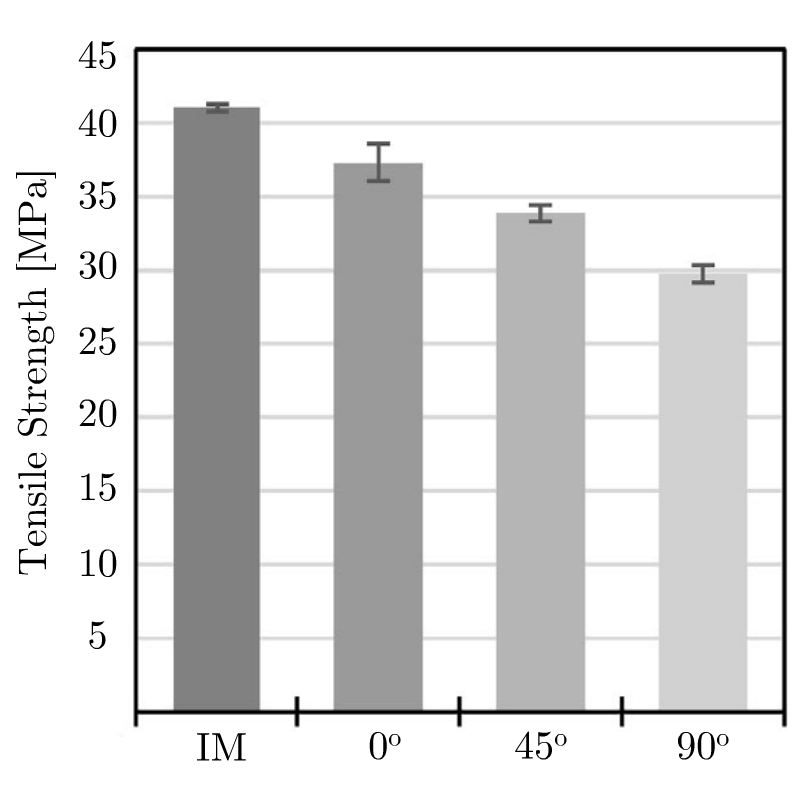
\includegraphics[height=6cm, keepaspectratio]{lit_mechpropFFF}
	}
	\hfill
	\subfloat[Representation of coupons used\label{fig:KochRes}]{%
		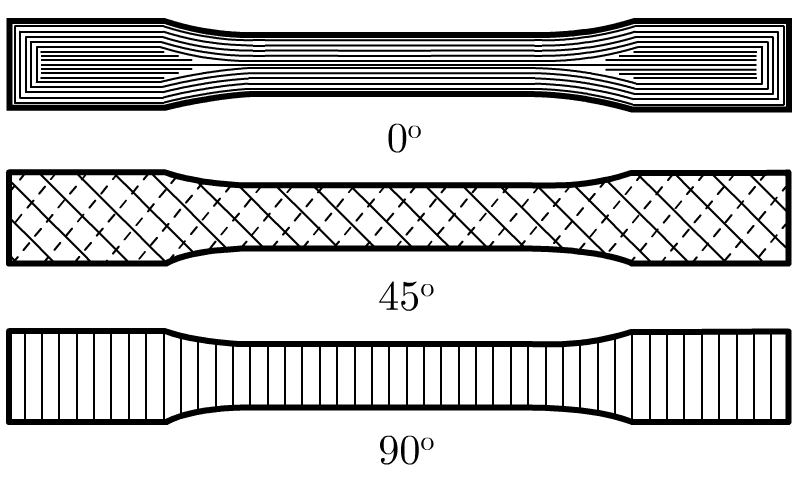
\includegraphics[height=4cm, keepaspectratio]{lit_mechpropFFF2}
	}
	\caption{Results from Koch \emph{et al.} \cite{Koch2017}} \label{fig:FFFmechProp}
\end{figure}

\section{Failure Criteria}\label{sec:FC}   
The increased use of advanced materials in industry has brought upon a necessity to properly characterize their strengths and failure modes. Composites in particular are commonly used in highly demanding engineering fields given that they excel in mechanical properties. However, due to their nature, their behavior is extremely anisotropic. For this reason, it has been of great interest to develop a proper way to model the behavior of anisotropic materials under mechanical stresses as a way to predict part failure \textendash~a practice from here on referred to as developing a \emph{failure criterion}. 

Early attempts to properly predict failure of anisotropic materials go as far back as 1948 with the Hill model \cite{Osswald2017a}. Further developments led to a plethora of failure criteria, such as the Tsai-Hill, Malmeister, Tsai-Wu, Gol'denblat-Kopnov, Puck, and Cuntze to name a few \cite{Osswald2017a,Osswald2015}. A wide variety of criteria exists because a model will rarely capture the complete failure behavior of an anisotropic material. To illustrate this point, refer to Figure \ref{fig:FCComp}, reproduced from work by Sun \emph{et al}. \cite{Sun1996} where a composite glass fiber and epoxy laminate was loaded biaxially, in a direction that was either parallel ($\sigma_{11}$), perpendicular ($\sigma_{22}$) to the fiber, or a combination of both. Positive stresses indicate tensile load, while negative values point to compressive forces. The data, represented by the white squares, does not agree with any of the used models in the fourth quadrant of the graph. This type of behavior is common throughout the literature: Puck's model is great at predicting shear strengthening effects, but doesn't perform well when dealing with combined axial loading scenarios; the Gol'denblat-Kopnov model by contrast is great at predicting axial stress interactions, but falls short when dealing with shear strengthening effects caused by combined shear-axial loadings. These trends point to the limitations of each model: in order to either facilitate calculations, or due to the difficulty of performing combined loading tests, interaction effects are neglected either by mathematical choice, or indirectly through the inner workings of the failure criterion \cite{Osswald2017a}.  

\begin{figure}[h]
	\center
	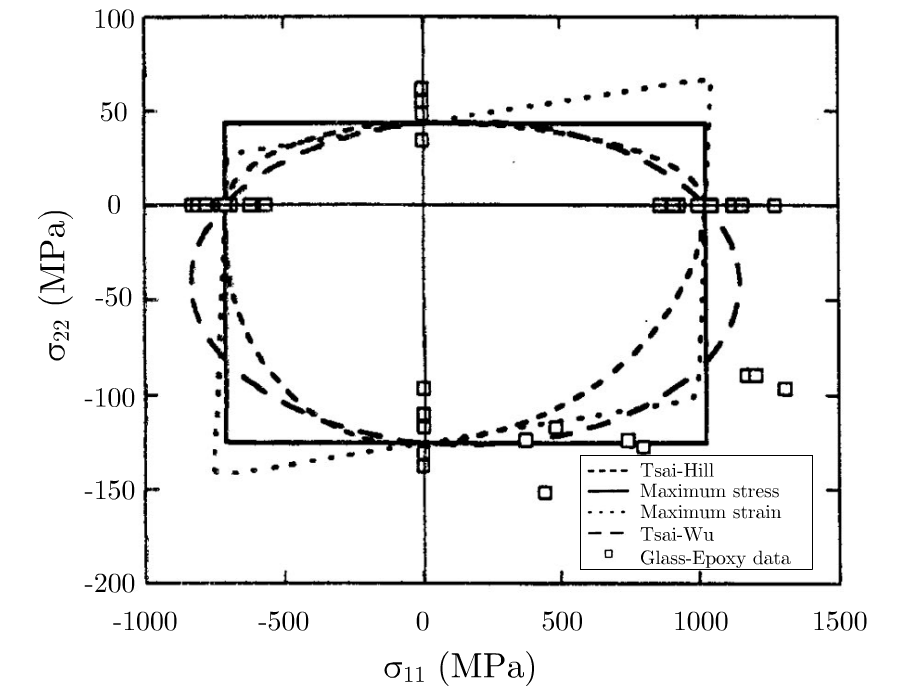
\includegraphics[height=10cm, keepaspectratio]{FC_comparison}
	\caption{Comparison of different failure criteria. \cite{Sun1996}} \label{fig:FCComp}
\end{figure}     

Properly mapping a failure surface through a criterion proves to be an invaluable tool for design, since it allows engineers to assess if a part will perform safely under its intended loading conditions. Such tool could help overcome the main shortcoming of FFF, since a failure envelope would allow proper part design considerations. Chapter \ref{ch:oocrit} describes in detail an approach based on the Gol'denblat-Kopnov model that includes interaction effects to properly describe the failure behavior of anisotropic parts, as well as showing examples of how it has been applied to describe failure in AM parts, with the FFF technique in particular receiving larger emphasis. 
% Nomenclature introduced in this chapter:
\nomenclature[A]{SLA}{Stereolithography}% 
\nomenclature[A]{SLS}{Selective Laser Sintering}%
\nomenclature[A]{$\mu$CT}{Micro Computer Tomography}%

% Symbols introduced in this chapter:
\nomenclature[S]{$\sigma$}{Axial stress \nomunit{$MPa$}}
\nomenclature[S]{$\tau$}{Shear stress \nomunit{$MPa$}}
\nomenclature[S]{$\sigma_{11}$}{Axial stress in the 1-1 direction \nomunit{$MPa$}}
\nomenclature[S]{$\sigma_{22}$}{Axial stress in the 2-2 direction \nomunit{$MPa$}}
\nomenclature[S]{$\sigma_{33}$}{Axial stress in the 3-3 direction \nomunit{$MPa$}}
\nomenclature[S]{$\tau_{12}$}{Shear stress in the 1-2 plane \nomunit{$MPa$}}
\nomenclature[S]{$\tau_{13}$}{Shear stress in the 1-3 plane \nomunit{$MPa$}}
\nomenclature[S]{$\tau_{23}$}{Shear stress in the 2-3 plane \nomunit{$MPa$}}
\end{document}
                %% oocriterion.tex
\documentclass[main.tex]{subfiles}
\begin{document}
\chapter{Previous work} \label{ch:oocrit}


The SSIC offers a way of capturing in a more accurate manner the different failure modes of parts produced through AM technologies. As an example, the model has been successfully implemented by Obst \emph{et al.} in 2018 for SLS manufactured parts produced with PA12 \cite{Obst2018, Obst2017}. Their results show how the model was able to capture the $\tau_{12}$-$\sigma_{22}$ and $\sigma_{11}$-$\sigma_{22}$ interactions. The failure surface obtained, shown in Figure \ref{fig:OOCSLS}, was able to capture the interactions between certain axial and transverse stresses. However, due to the limitations of the SLS process, it was not possible to measure the interaction slope between the $\tau_{12}$ and $\sigma_{11}$ directions.

\begin{figure}[h]
	\center
	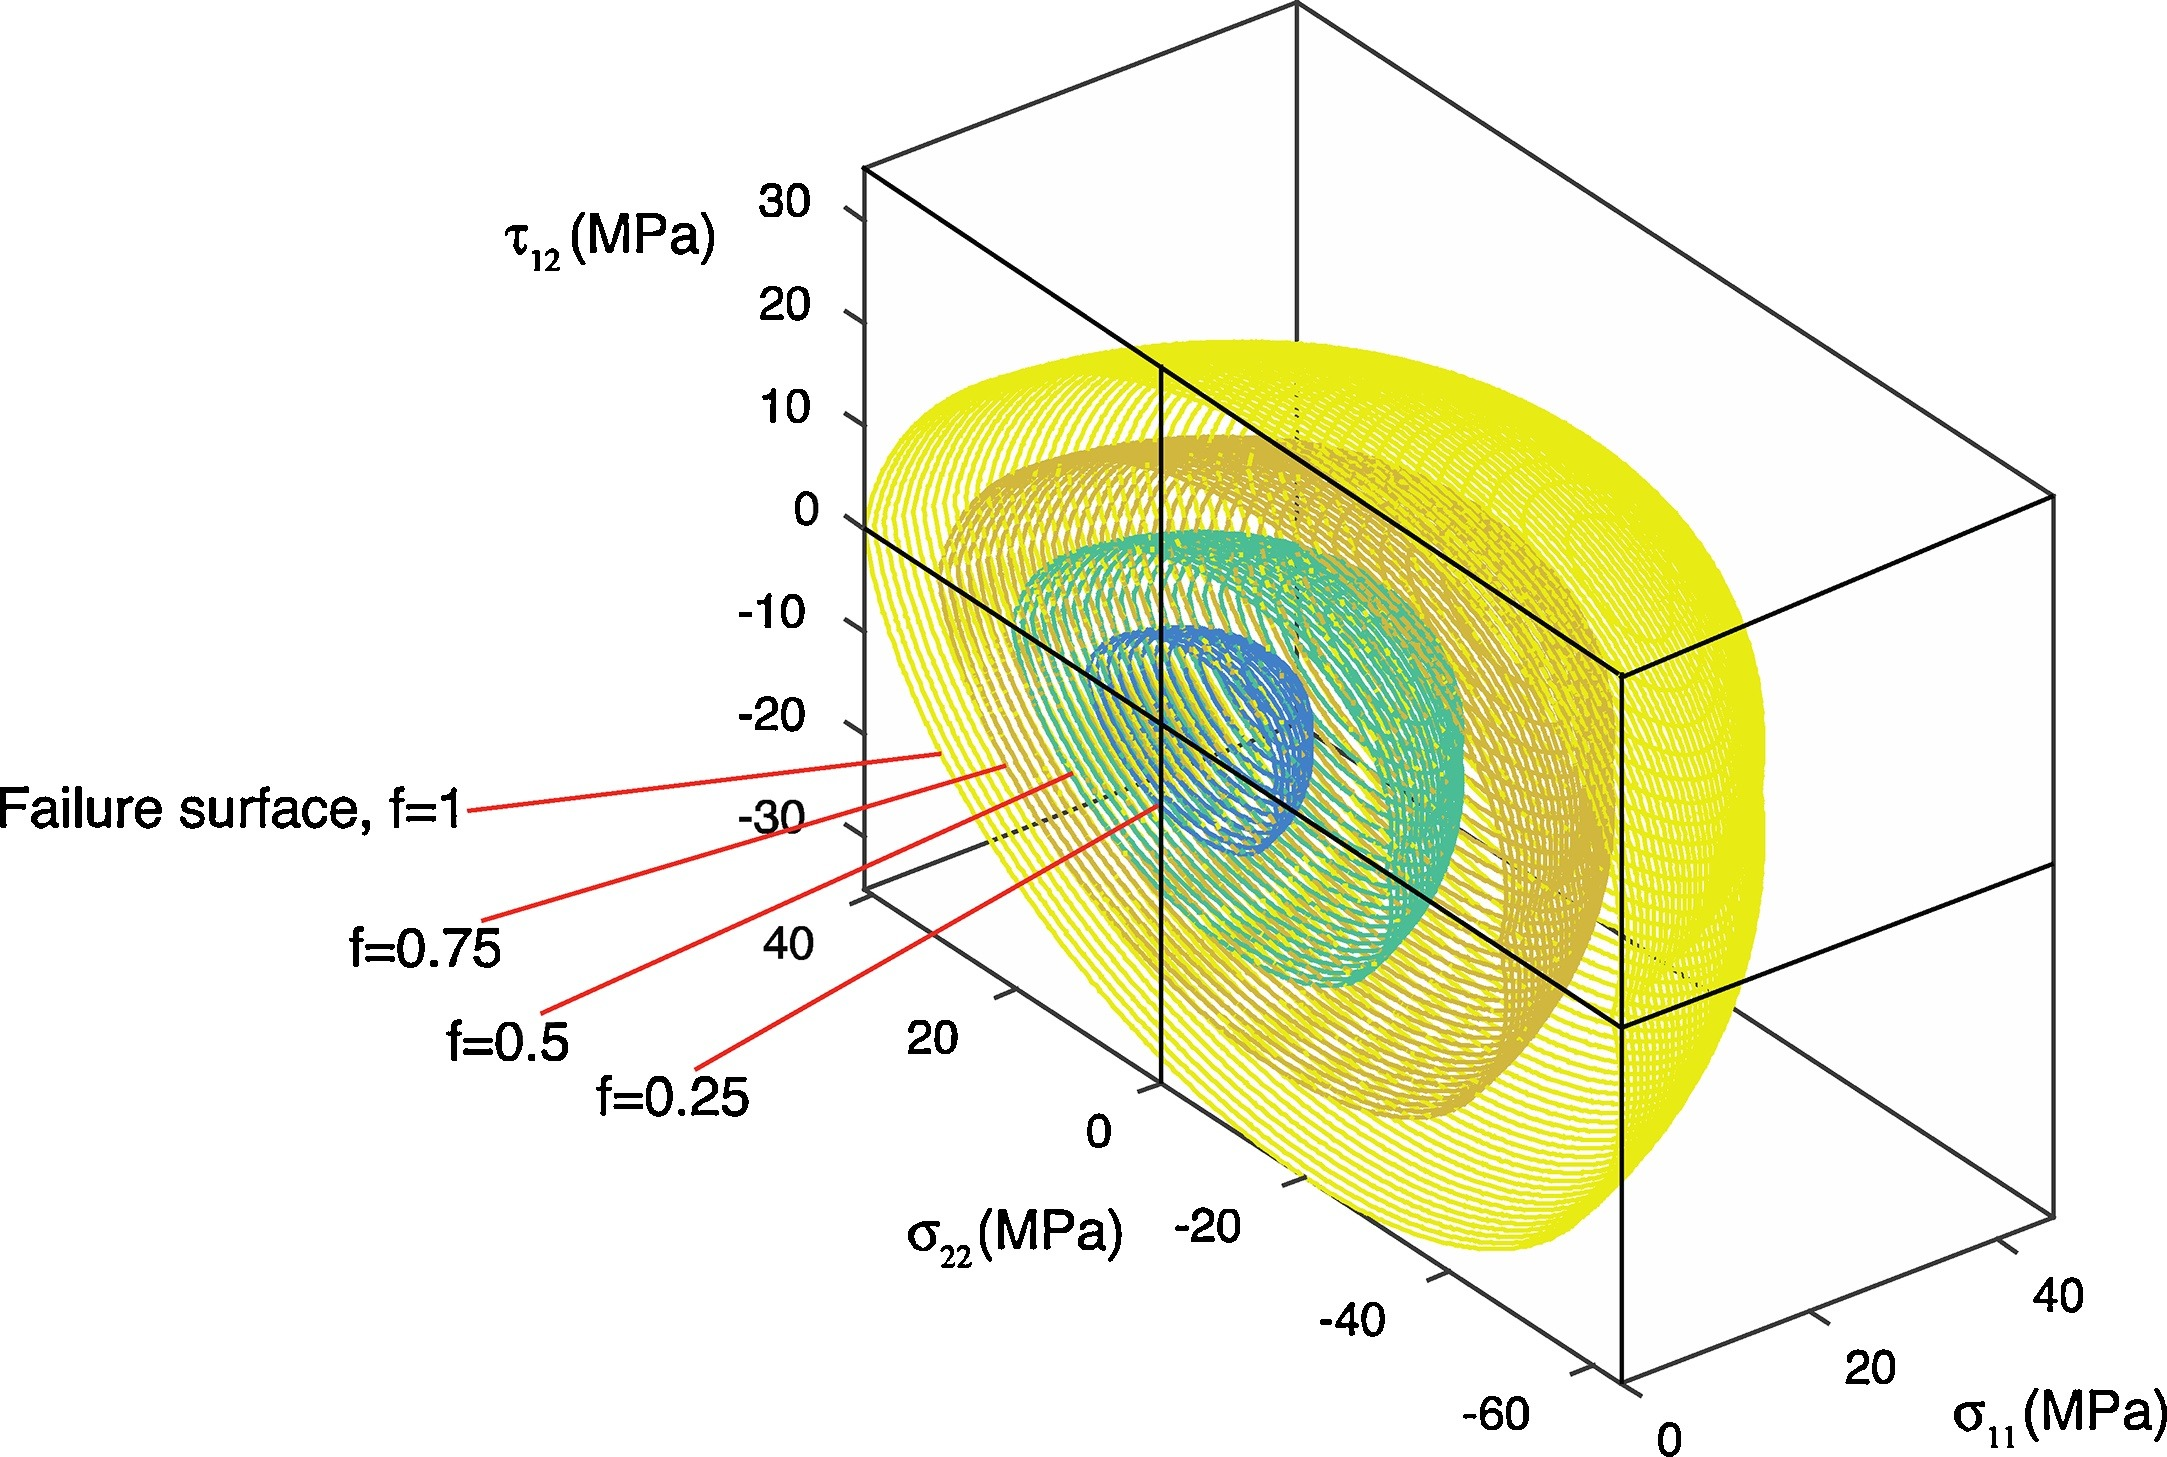
\includegraphics[height=6cm]{Obst_SLS}
	\caption{Failure surface for SLS developed through the SSIC \cite{Obst2018}} \label{fig:OOCSLS}
\end{figure}

Recent unpublished work by Osswald \emph{et al.} \cite{Osswald2020} generated a failure envelope for Multi-Jet Fusion (MJF) parts produced using PA12, and compared it to the surface obtained by Obst \emph{et al.} \cite{Obst2018}. Results indicate that, while both techniques are based on Powder Based Fusion (PBF) and use the same material, the envelopes for each AM technology were distinct, serving as proof that these technologies are not as comparable under complex loading conditions as previously assumed. The transverse-axial interaction for the MJF case was significantly less pronounced than for SLS, further reinforcing that each AM technique needs to be studied in a case-by-case basis in terms of mechanical failure characterization. 

\begin{figure}[!htbp]
	\center
	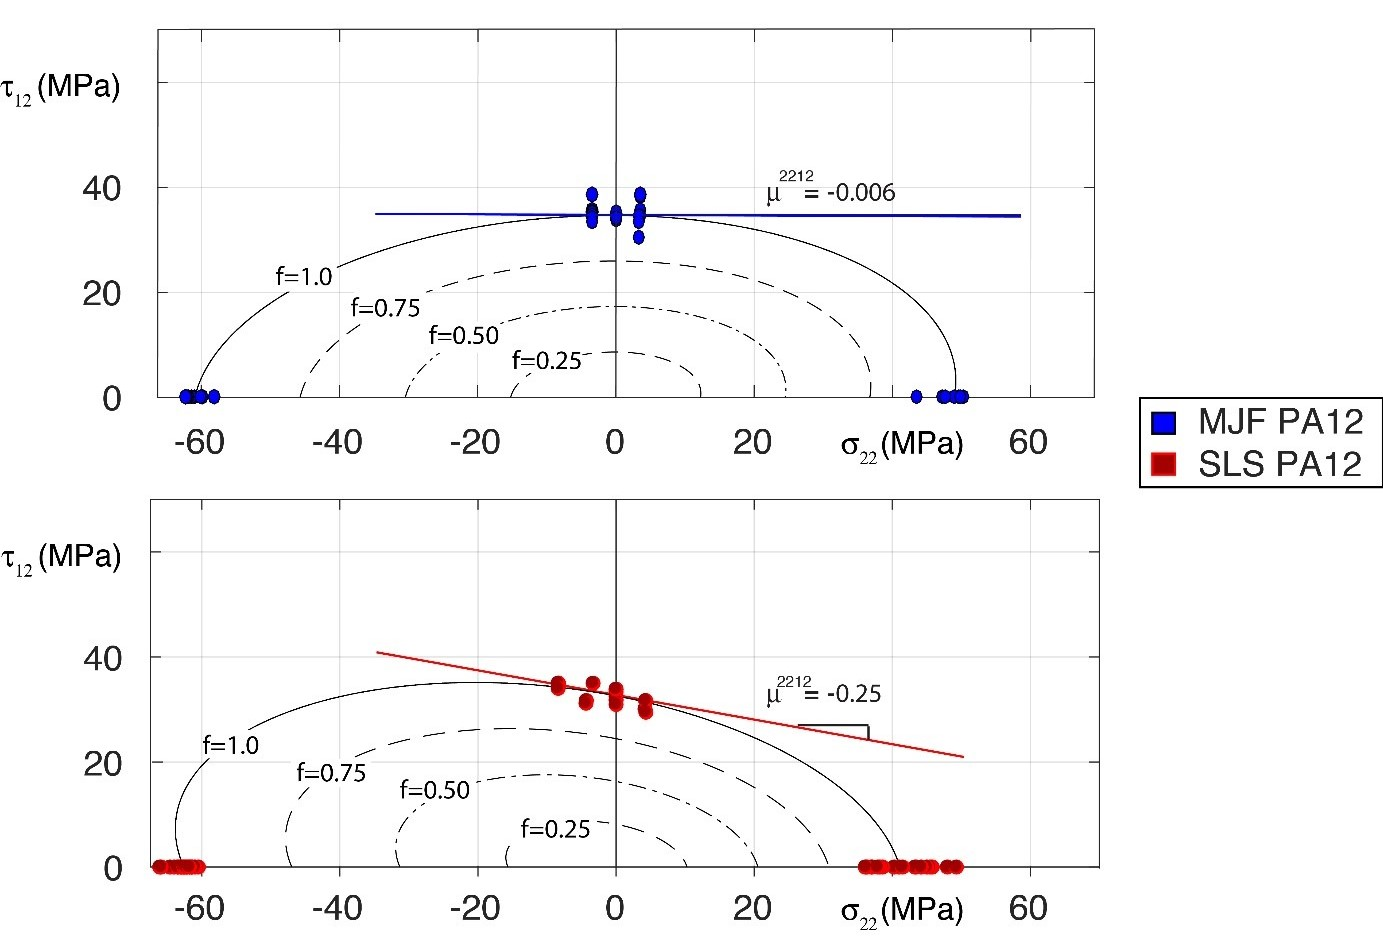
\includegraphics[height=10cm]{pbfcomp}
	\caption{Comparison of the $\sigma_{22} - \tau_{12}$ interaction for SLS and MJF PA12 parts \cite{Osswald2020}} \label{fig:pbfcomp}
\end{figure}

\section{Development of SSIC envelope for FFF parts}\label{sec:SSICFFF}

In 2019, Mazzei Capote \emph{et al.} \cite{MazzeiCapote2019} developed a failure envelope for FFF parts produced using a customized ABS filament produced in-house. Specimens were produced using either a commercially available desktop FFF printer (Lulzbot TAZ5, USA), or a customized 6-axis robotic printing solution whenever the bead orientation was hard to achieve using a \emph{2.5-D} machine. The robotic printer was based on a 6-axis robot (ABB IRB-120, Switzerland) and fitted with a stationary printhead mounted on an aluminum frame, chosen to be the same extruder from the traditional printer (LulzBot TAZ Single Extruder Tool Head v2, 0.5 mm nozzle, USA) to minimize machine influence on the results \cite{VanHulle2017}. The final surface obtained showed significant stress interactions in certain directions. Starting with the $\sigma_{11}$-$\sigma_{22}$ plane, it can be seen that the failure envelope has a slight tilt. Refer to Figure~\ref{fig:1122plane} for a graph showing the calculated failure envelope, including the experimental data for reference. This tilt is evidence of an interaction between the transverse and longitudinal stresses. The conclusion is that FFF parts produced with the print parameters used in the study should show strengthening when loaded bi-axially in compression.

\begin{figure}[h]
	\center
	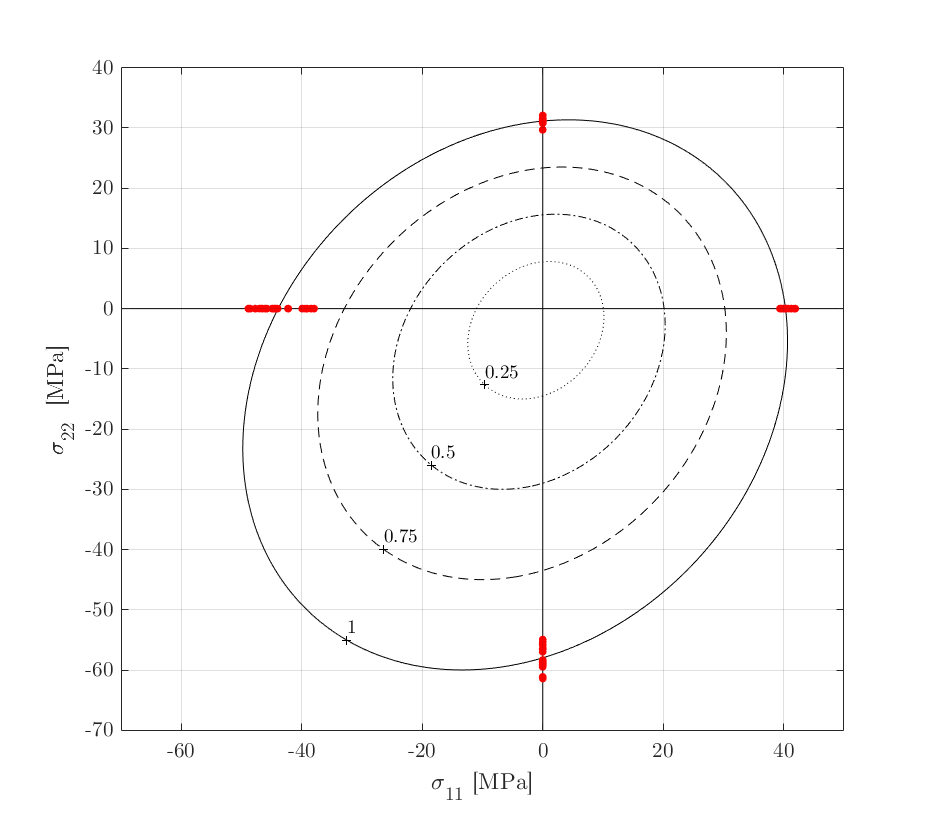
\includegraphics[width=\linewidth, keepaspectratio]{11_22plane}
	\captionsetup{justification=centering} %long caption
	\caption[failure envelope in the $\sigma_{11}$-$\sigma_{22}$ plane]{$\sigma_{11}$-$\sigma_{22}$ plane including data for reference.} \label{fig:1122plane}
\end{figure}

\pagebreak

Using the results from combined loading tests plotted in the $11-12$ and $22-12$ planes allows visualization of the transverse-axial stress interactions. Beginning with the $11-12$ plane, it can be seen that the calculated interaction slope $\mu^{1112}$ equals $5.2\times 10^{-3}$, a value that's practically zero. Using this parameter, the failure surface shown in Figure \ref{fig:1112plane} can be obtained. A dashed line representing $\mu^{1112}$ is added for reference. The $22-12$ plane by comparison reveals a considerable slope. It can be seen through the use of combined loads that there is a slight decrease in the shear strength of the specimens when a tensile load is applied in the $2-2$ direction. A slope of -0.2 was obtained for $\mu^{2212}$. Figure \ref{fig:2212plane} shows the resulting surface with the data and a line with a slope of -0.2 overlaid for reference.

\pagebreak

\begin{figure}[h]
	\center
	\subfloat[failure envelope in the $\sigma_{11}$-$\tau_{12}$ plane\label{fig:1112plane}]{%
		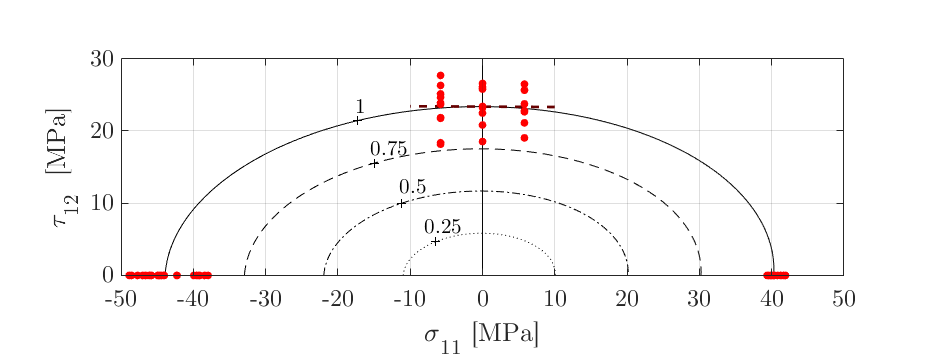
\includegraphics[width=0.9\linewidth, keepaspectratio]{11_12plane}
	}
	\linebreak
	\subfloat[failure envelope in the $\sigma_{22}$-$\tau_{12}$ plane\label{fig:2212plane}]{%
		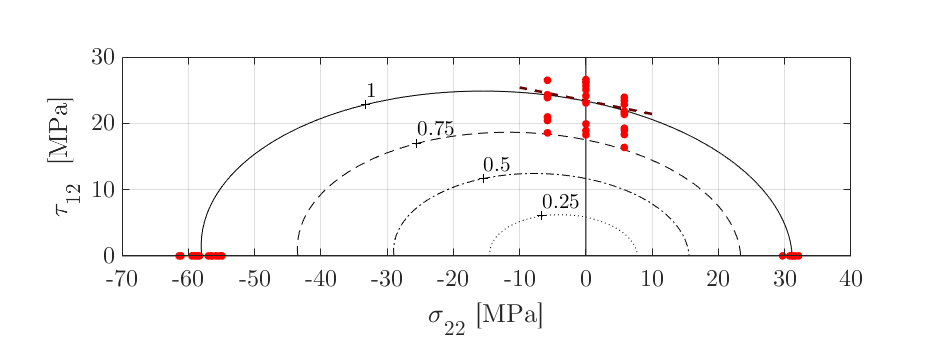
\includegraphics[width=0.9\linewidth, keepaspectratio]{22_12plane}
	}
	\caption{Comparison of interaction slopes in the axial-transverse stress planes} \label{fig:SSIcomp}
\end{figure}

\section{Validation of the FFF Failure envelope}\label{sec:FFFval}

The validity of the envelope described in Section \ref{sec:SSICFFF} was tested by Mazzei Capote  \emph{et al.} \cite{MazzeiJCompSci} in 2019. In this study, the failure function was used to estimate the failure stress of mechanical coupons loaded under tension, with a variety of raster angles being used to generate a complex loading state in the local coordinate system. Results indicated the failure prediction boundary was within 5 to 10\% of the real value. Results are summarized in Figure \ref{fig:jcompscir}, where the average of 5 mechanical tests per raster angle is represented in a dot, and the SSIC predicted failure stress is shown in a bright red line. These are compared to simpler FC, such as the maximum stress criteria in the $\sigma_{11}$, $\sigma_{22}$, and $\tau_{12}$ directions, labeled M1-1, M2-2, and M1-2 respectively. 

\begin{figure}[!htbp]
	\center
	\subfloat[Loading \label{fig:complload}]{%
		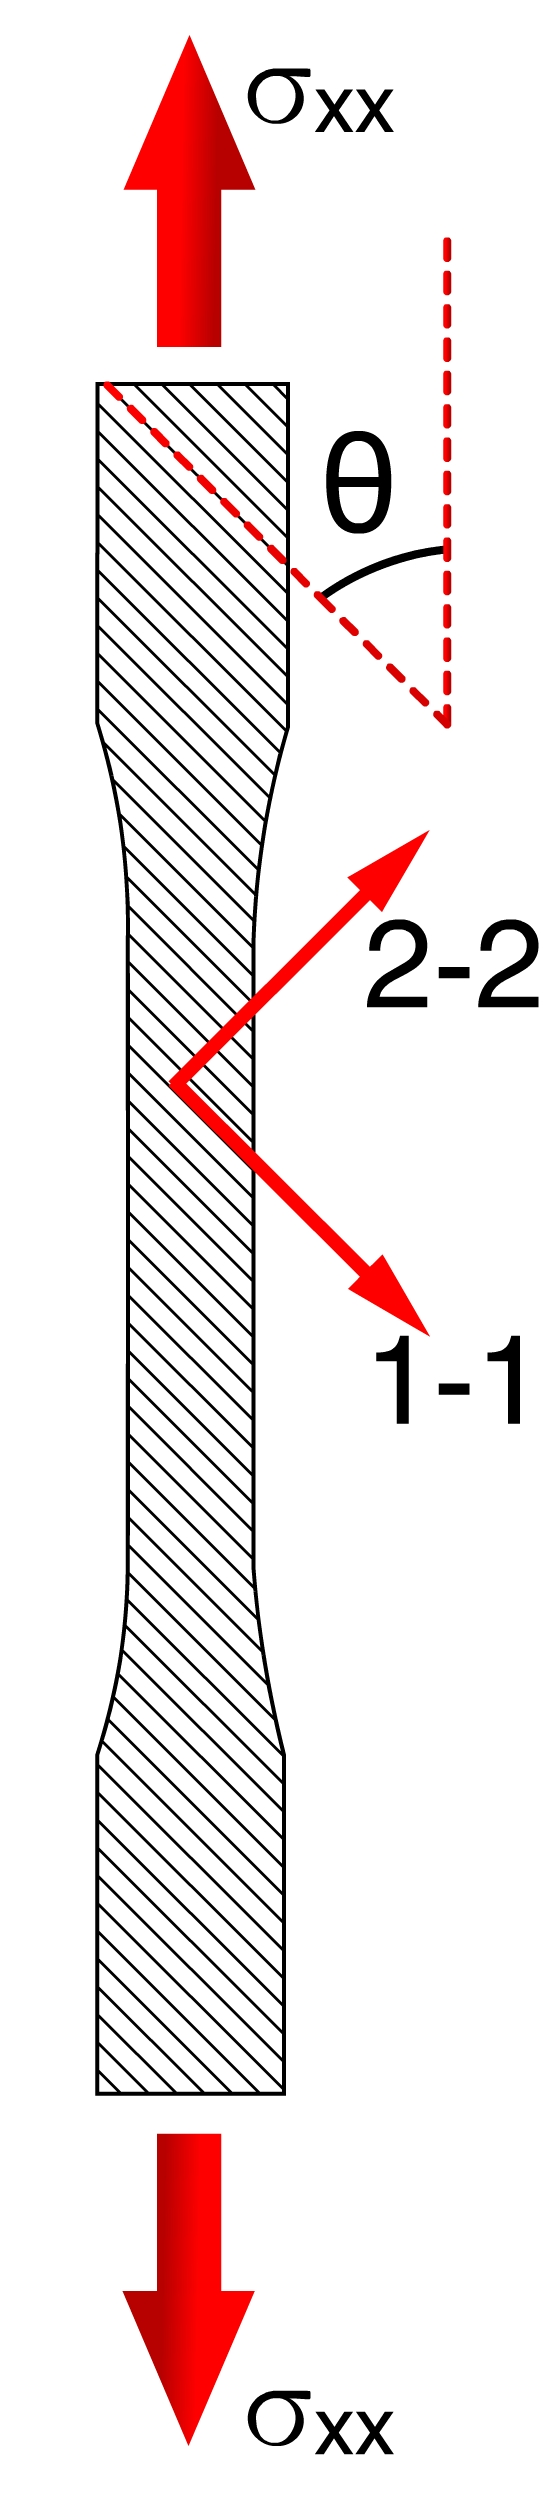
\includegraphics[height=9cm, keepaspectratio]{compl_load.jpg}
	}
	\hfill
	\subfloat[Comparison of data and failure prediction using various FC\label{fig:compsci}]{%
		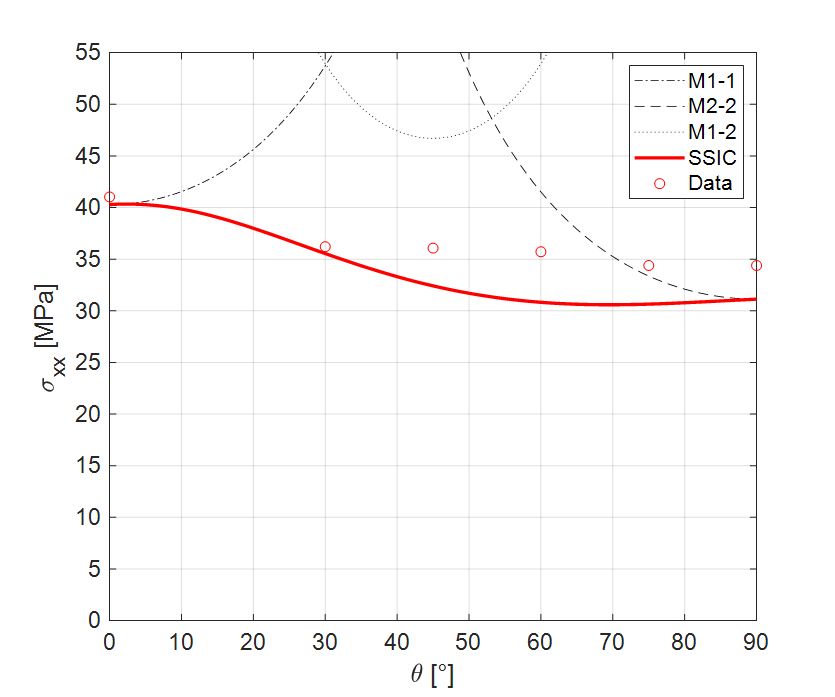
\includegraphics[height=9cm, keepaspectratio]{FC_comp.png}
	}
	\caption{Results from \cite{MazzeiJCompSci}} \label{fig:jcompscir}
\end{figure} 


While the use of FC in AM is promising, its adoption has been limited in scope. Part of the problem lies in the large number of mechanical tests required to achieve a trustworthy failure envelope, as well as the requirement of specialized equipment \textendash~such as a variety of mechanical testing devices, as well as specialized printing solutions as seen in the FFF failure envelope. Chapter \ref{ch:proposal} outlines proposed work aimed at predicting the mechanical response of FFF parts using machine learning methods. Some, if not all of the concepts explored could easily be extrapolated to other AM techniques. It should be noted that the two methods are not mutually exclusive. A combination of both FC and machine learning predictive methods can hopefully lead to a higher adoption rates of AM in industrial scenarios where the final desired application involves complex mechanical loads upon the finished part. 

% Nomenclature introduced in this chapter:
\nomenclature[A]{SSIC}{Stress-Stress Interaction Criterion}% 
\nomenclature[A]{GKC}{Gol'denblat-Kopnov Criterion}% 
\nomenclature[A]{MJF}{Multi-Jet Fusion}% 
\nomenclature[A]{PBF}{Powder Bed Fusion}% 

% Symbols introduced in this chapter:
\nomenclature[S]{$X_t$}{Tensile strength in the 1-1 direction \nomunit{$MPa$}}
\nomenclature[S]{$X_c$}{Compressive strength in the 1-1 direction \nomunit{$MPa$}}
\nomenclature[S]{$Y_t$}{Tensile strength in the 2-2 direction \nomunit{$MPa$}}
\nomenclature[S]{$Y_c$}{Compressive strength in the 2-2 direction \nomunit{$MPa$}}
\nomenclature[S]{$S$}{Shear strength in the 1-2 plane \nomunit{$MPa$}}
\nomenclature[S]{$S_{45p}$}{Positive shear strength for 45$^\circ$ specimen \nomunit{$MPa$}}
\nomenclature[S]{$S_{45n}$}{Negative shear strength for 45$^\circ$ specimen \nomunit{$MPa$}}
\nomenclature[S]{$\mu^{1112}$}{SSIC parameter- slope at pure shear failure in the $\sigma_{11}$ - $\tau_{12}$ plane \nomunit{$-$}}
\nomenclature[S]{$\mu^{2212}$}{SSIC parameter- slope at pure shear failure in the $\sigma_{22}$ - $\tau_{12}$ plane \nomunit{$-$}}
\end{document}
                %\include{experimental}
                %\include{results}
                %\include{conclusions}
%               \include{examples}

		%Create Bibliography
		\cleardoublepage
        \phantomsection
		\addcontentsline{toc}{chapter}{Bibliography}
		\printbibliography

        %Create Appendices
		\appendix
			%\include{mg94}
			%\pagestyle{fancy}
			%\include{fsurfcode}
			%\include{data}
			%\include{surf}
			


        
\end{document}
